%
% bilanz.tex -- Bilanz-Modelle
%
% (c) 2018 Prof Dr Andreas Müller, Hochschule Rapperswil
%
\section{Strahlungsbilanzmodelle\label{skript:section:budyko}}
\rhead{Strahlunbsbilanzmodelle}
Im Kapitel~\ref{chapter:wetter und klima} haben wir die physikalischen
Grundlagen der Wetter und Klimaphänomene studiert.
In diesem Abschnitt wollen wir ein einfaches Modell für die Energiebilanz
der Erde entwickeln.

\subsection{Strahlungsbilanz\label{skript:subsection:strahlungsbilanz}}
Wir formulieren ein Modell mit einer einzigen Variablen, der globalen
Mitteltemperatur $T$.
Berechnet werden soll die zeitliche Entwicklung von $T$.

\subsubsection{Einstrahlung}
Die Erde mit Radius $R$ erhält ihre Energie von der Sonne, die
den konstanten Energiefluss $S_0 = 1368 \text{W\,m}^{-2}$
einstrahlt.
Der Querschnitt der Erde ist $\pi R^2$, auf den eine Leistung von
$\pi R^2 S_0$ fällt.
Die Atmosphäre und die Weltmeere transportieren diese Energie, wir nehmen
an, dass sie gleichmässig über die ganze Erdoberfläche verteilt wird.
Die pro Flächeneinheit anfallende Leistung ist daher
\begin{equation}
\frac{\pi R^2 S_0}{4\pi R^2} = \frac14S_0=Q.
\label{skript:bilanz:einstrahlung}
\end{equation}

Doch kann nicht die gesamte Energie absorbiert werden.
Ein Teil wird von Wolken oder von Eis an der Oberfläche 
gleich wieder reflektiert, aber auch Landmassen und die Meere reflektieren
einen kleineren Teil der Strahlung.
Die auf Seite~\pageref{skript:subsubsection:albedo} beschriebene Albedo
hat für die Erde Werte zwischen $0.3$ und $0.7$ je nach dem Grad der
Bewölkung und der Vereisung.
Bei tieferer Temperatur muss mit stärkerer Vereisung und mehr Wolken
gerechnet werden.
Sei $\alpha(T)$ die Albedo der Erde bei der Temperatur $T$.
Der von der Erde absorbierte Fluss ist daher
\begin{equation}
(1-\alpha(T)) Q.
\label{skript:bilanz:ausstrahlung}
\end{equation}
Die Grösse $1-\alpha(T)$ heisst auch die {\em Coalbedo}.
\index{Coalbedo}%

\subsubsection{Ausstrahlung}
Die Erde verliert Energie auch wieder durch Strahlung.
Nach dem Stefan-Boltzmannschen Gesetz~\eqref{skript:stefon-boltzmann}
ist die Ausstrahlung der Erde proportional zur vierten Potenz der
Temperatur, also $T^4$.

\subsubsection{Bilanzgleichung}
Die Temperatur ändert sich umso mehr, je grösser das Ungleichgewicht
zwischen Einstrahlung \eqref{skript:bilanz:einstrahlung} und
\eqref{skript:bilanz:ausstrahlung} ist.
Die Wärmekapazität der Erdoberfläche spielt ebenfalls
eine Rolle, je grösser diese ist, desto träger folgt die Temperatur dem
Energiebilanzüberschuss.

Wir erhalten so die Differentialgleichung
\begin{equation}
C\frac{dT}{dt}
=
(1-\alpha(T)) Q - \sigma T^4.
\label{skript:bilanz:basic}
\end{equation}
Je grösser $C$ ist, desto kleiner ist die Änderungsgeschwindigkeit der
globalen Mitteltemperatur bei gleicher rechter Seite.

\subsubsection{Gleichgewichtslösung}
Wir suchen eine Gleichgewichtslösung für dieses Modell, und nehmen zu diesem
Zweck den typischen Wert $\alpha=0.3$ der Albedo der Erde.
Sie muss $\dot T=0$ erfüllen, also
\begin{align*}
(1-\alpha) Q -\sigma T^4 &=0
\\
\Rightarrow
\qquad
T&=\root 4\of{\frac{(1-\alpha)Q}{\sigma}}
\end{align*}
Setzt man die üblichen Werte für $Q$ ein, erhält man eine globale
Mitteltemperatur von $T=254.8\,\text{K}$.

\subsubsection{Treibhauseffekt}
Die tatsächliche global Mitteltemperatur $T=287.7\,\text{K}$ ist.
Diese Diskrepanz ist zwei Unzulänglichkeiten diesen einfachen
Modells zurückzuführen:
\begin{enumerate}
\item
Der Treibhauseffekt sorgt dafür, dass nur ein Teil der abgestrahlten
Wärmestrahlung die Erde tatsächlich verlässt.
Wir können dies dadurch modellieren, dass wir in der Gleichung
\eqref{skript:bilanz:basic} den Ausstrahlungsterm um einen Faktor
$\varepsilon$ reduzieren, der den Treibhauseffekt modellieren soll.
Die neue Grundgleichung wird dann
\begin{equation}
C\frac{dT}{dt}
=
(1-\alpha(T)) Q - \varepsilon\sigma T^4.
\label{skript:bilanz:basic2}
\end{equation}
Um die aktuelle Gleichgewichtstemperatur $T=287.7\,\text{K}$ von 2010
zu reproduzieren müssen wir $\varepsilon=0.32$ wählen.
\item
Die Albedo hängt von der Temperatur ab und wird mit abnehmender 
Temperatur grösser.
Bei sehr tiefen Temperaturen kann die Albedo auf bis $0.7$ steigen.
Ein einfaches Modell,
welches diesen Sachverhalt abbildet, ist
\begin{equation}
\alpha(T)=0.5-0.2\tanh\biggl(\frac{T-265}{10}\biggr).
\label{skript:bilanz:albedo}
\end{equation}
Die ist zwar etwas willkürlich, trifft die Realität aber qualitativ nicht
schlecht.
\end{enumerate}
Das Modell mit der Albedo-Funktion~\eqref{skript:bilanz:albedo}
hat nicht nur einen sondern drei Gleichgewichtspunkte.
Die Einstrahlung und die Ausstrahlung ist in
Abbildung~\ref{skript:bilanz:modellbild} dargestellt.

\subsubsection{Gleichgewichte}
\begin{figure}
\centering
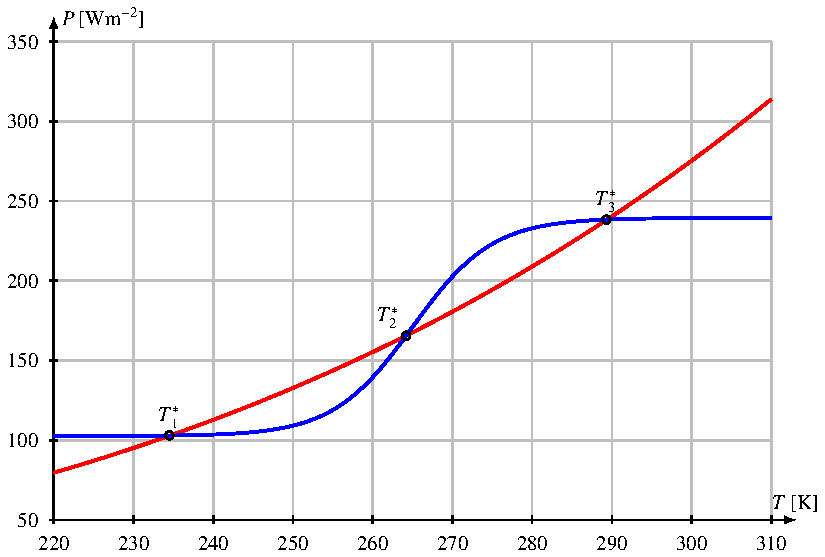
\includegraphics{chapters/5/bilanzmodell.pdf}
\caption{Einstrahlung und Ausstrahlung in dem einfachen Bilanzmodell
mit der Modellgleichung
\eqref{skript:bilanz:basic2} und der Albedo-Funktion
\eqref{skript:bilanz:albedo}.
Die Ausstrahlung $\varepsilon\sigma T^4$ ist rot eingezeichnet,
blau ist die Ausstrahlung.
Es entstehen drei Gleichgewichtspunkte $T_1^*$, $T_2^2*$ und $T_3^*$,
von denen aber $T_2^*$ nicht stabil ist.
\label{skript:bilanz:modellbild}}
\end{figure}
Die beiden Gleichgewichtspunkte $T_1^*$ und $T_3^*$ sind stabil.
In beiden Punkten ändert sich die absorbierte Energie kaum bei
einer Temperaturänderung, aber die Ausstrahlung wird bei erhöhter 
Temperatur wesentlich effizienter, so dass sich die Erde wieder
abkühlt.
Ebenso verringert sich die Ausstrahlung bei leicht tieferer Temperatur
sofort, so dass die Erde sich wieder zur Gleichgewichtstemperatur aufwärmen
kann.

Das Gleichgewicht $T_2^*$ ist dagegen nicht stabil.
Bei höherer Temperatur wird die Einstrahlung sofort grösser, ohne dass
die Ausstrahlung mithalten kann, so dass sich die Erde weiter
aufwärmt bis zur Temperatur $T_3^*$.
Bei leicht tieferer Temperatur steigt die Albedo stark an so dass die
Einstrahlung schnell abnimmt, während die Ausstrahlung nur vergleichsweise
langsam zurückgeht, die Erde kühlt sich bis auf die Temperatur $T_1^*$ ab.

\subsubsection{Bifurkation und globale Erwärmung}
\begin{figure}
\centering
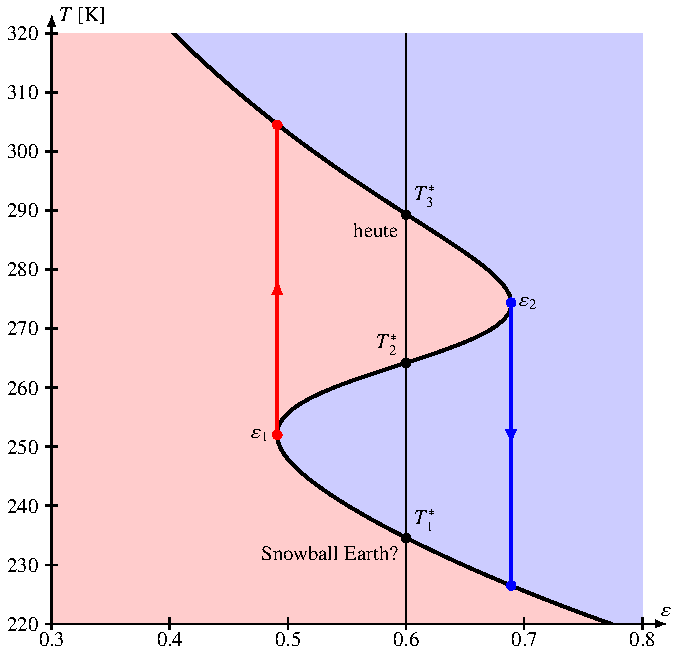
\includegraphics{chapters/5/bifurkation.pdf}
\caption{Phasendiagramm für das Bilanzmodell
\eqref{skript:bilanz:basic2}
in Abhängigkeit vom Treibhauseffekt-Parameter $\varepsilon$.
\label{skript:bilanz:bifurkation}}
\end{figure}
Der Parameter $\varepsilon$ modelliert den Treibhauseffekt.
Steigt die Konzentration der Klimagase in der Atmosphäre, wird die
abgestrahlten Leistung geringer, also $\varepsilon$ kleiner.
Es lohnt sich daher, die Entwicklung des Gleichgewichtspunkte in 
Abhängigkeit von $\varepsilon$ zu untersuchen.
Das Phasendiagramm des Modells
\eqref{skript:bilanz:basic2} in Abhängigkeit von $\varepsilon$
ist in Abbildung~\ref{skript:bilanz:bifurkation} dargestellt.

Man kann aus dem Diagramm ablesen, dass mit weiterer Zunahme des 
Treibhauseffektes, als mit Abnahme von $\varepsilon$, die globale
Mitteltemperatur weiter ansteigen wird.
Sinkt $\varepsilon$ unter den kritischen Wert $\varepsilon_1$ steigt die
Temperatur auf über $305\,\text{K}$.
In diesem Fall verschwinden die beiden Gleichgewichtspunkte $T_1^*$
und $T_2^*$, es bleibt nur das Gleichgewicht $T_3^*$.

Interessant ist aber auch, was bei starker Abnahme der
Treibhausgaskonzentration passiert.
Wenn $\varepsilon$ über $\varepsilon_2$ ansteigt, dann verschwinde
$T_3^*$ und $T_2^*$, es bleibt nur der Gleichgewichtspunkt $T_1^*$,
bei dem die ganze auf sehr tiefer Temperatur vereist.
Man vermutet, dass genau dieser Zustand in der Phase des {\em Snowball Earth}
eingetreten ist, als die ersten photosynthetisierenden Organismen die
Treibhausgase dramatisch reduziert und damit $\varepsilon$ stark
erhöht hatten.
Man beachte, dass es nur möglich ist, den heutigen Zustand wieder zu 
erreichen, indem die Treibhausgaskonzentration soweit gesteigert
wird, dass $\varepsilon<\varepsilon_1$ wird.
Es muss im Laufe der Erdgeschichte also nach der Snowball Earth Phase
auch Phasen mit wesentlich höherer Treibhausgaskonzentration als heute
gegeben haben.
Es ist denkbar, dass grosse Vulkanausbrüche genügend $\text{CO}_2$ in die
Atmosphäre gebracht haben, umd diesen Übergang zu erzwingen.

\subsection{Modell von Budyko\label{subsection:modell von budyko}}
Bisher haben wir die Ausstrahlung mit Hilfe des Stefan-Boltzmannschen
Gesetzes für die Strahlung eines schwarzen Körpers modelliert.
Es ist fraglich, ob dies tatsächlich zutreffend ist.
Die Ausstrahlung $E_\text{out}(T)$ der Ausstrahlung könnte also durchaus
eine kompliziertere Funktion sein.
Sie muss aber so beschaffen sein, dass sich bei der aktuellen
Mitteltemperatur $T^*$ ein stabiles Gleichgewicht ergibt.
In der Umgebung des Gleichgewichtes kann die Funktion $E_\text{out}(T)$
als lineare Funktion
$E_\text{out}= A+BT$
dargestellt werden.
Nahe bei $T^*$ kann die globale Mitteltemperatur also mit einem Modell
der Form
\begin{equation}
C
\frac{dT}{dt}
=
(1-\alpha(T)) Q- (A+BT)
\end{equation}
beschrieben werden.
Das Gleichgewicht erfüllt
\[
(1-\alpha(T^*))Q=A+BT^*
\] 
und ist stabil, wenn die Steigung der Einstrahlung kleiner ist als die
Die Steigung der Ausstrahlung, also
\begin{equation}
-Q\alpha'(T)
<
B.
\label{skript:budyko:cond}
\end{equation}
Dieses Modell wurde schon in den sechziger Jahren von Budyko vorgeschlagen.
Zahlenwerte für $A$ und $B$ konnten seit der damaligen Zeit durch
Satellitenbeobachtungen bestimmt werden.

Die Folgen des Treibhauseffektes sind auch in diesem einfacheren Modell
nachvollziehbar.
Die Erhöhung der Treibhausgaskonzentration reduziert die Ausstrahlung,
was sich zum Beispiel in einem kleineren Wert von $B$ äussert.
Eine Abnahme von $B$ um $\Delta B$ führt zu einer
Änderung der Gleichgewichtstemperatur um $\Delta T$, die die Gleichung
\begin{align*}
(1-\alpha(T^*+\Delta T))Q
&=
A + (B-\Delta B)(T^*+\Delta T)
\\
\underbrace{(1-\alpha(T^*))Q}_{\displaystyle=A+BT^*}
-Q\alpha'(T^*)\Delta T
&=
A+BT^*
- T^*\Delta B
+B\Delta T
\\
(Q\alpha'(T^*)
+
B)\Delta T
&=
T^*
\Delta B
\\
\Delta T
&=
\frac{T^*\Delta B}{Q\alpha'(T^*)+B}
\end{align*}
erfüllt.
Man kann daraus ablesen, dass eine Abnahme von $B$ genau dann zu einer
Zunahme der Mitteltemperatur, wenn der Nenner positiv ist, also
\[
Q\alpha'(T^*)+B > 0
\qquad\Rightarrow\qquad
-Q\alpha'(T^*)<B,
\]
was die Bedingung
\eqref{skript:budyko:cond}
beweist.




